The following visualizations was carried out using Matplotlib \cite{Matplotlib}.

\section{Class Distribution}
\begin{figure}[h!]
    \centering
    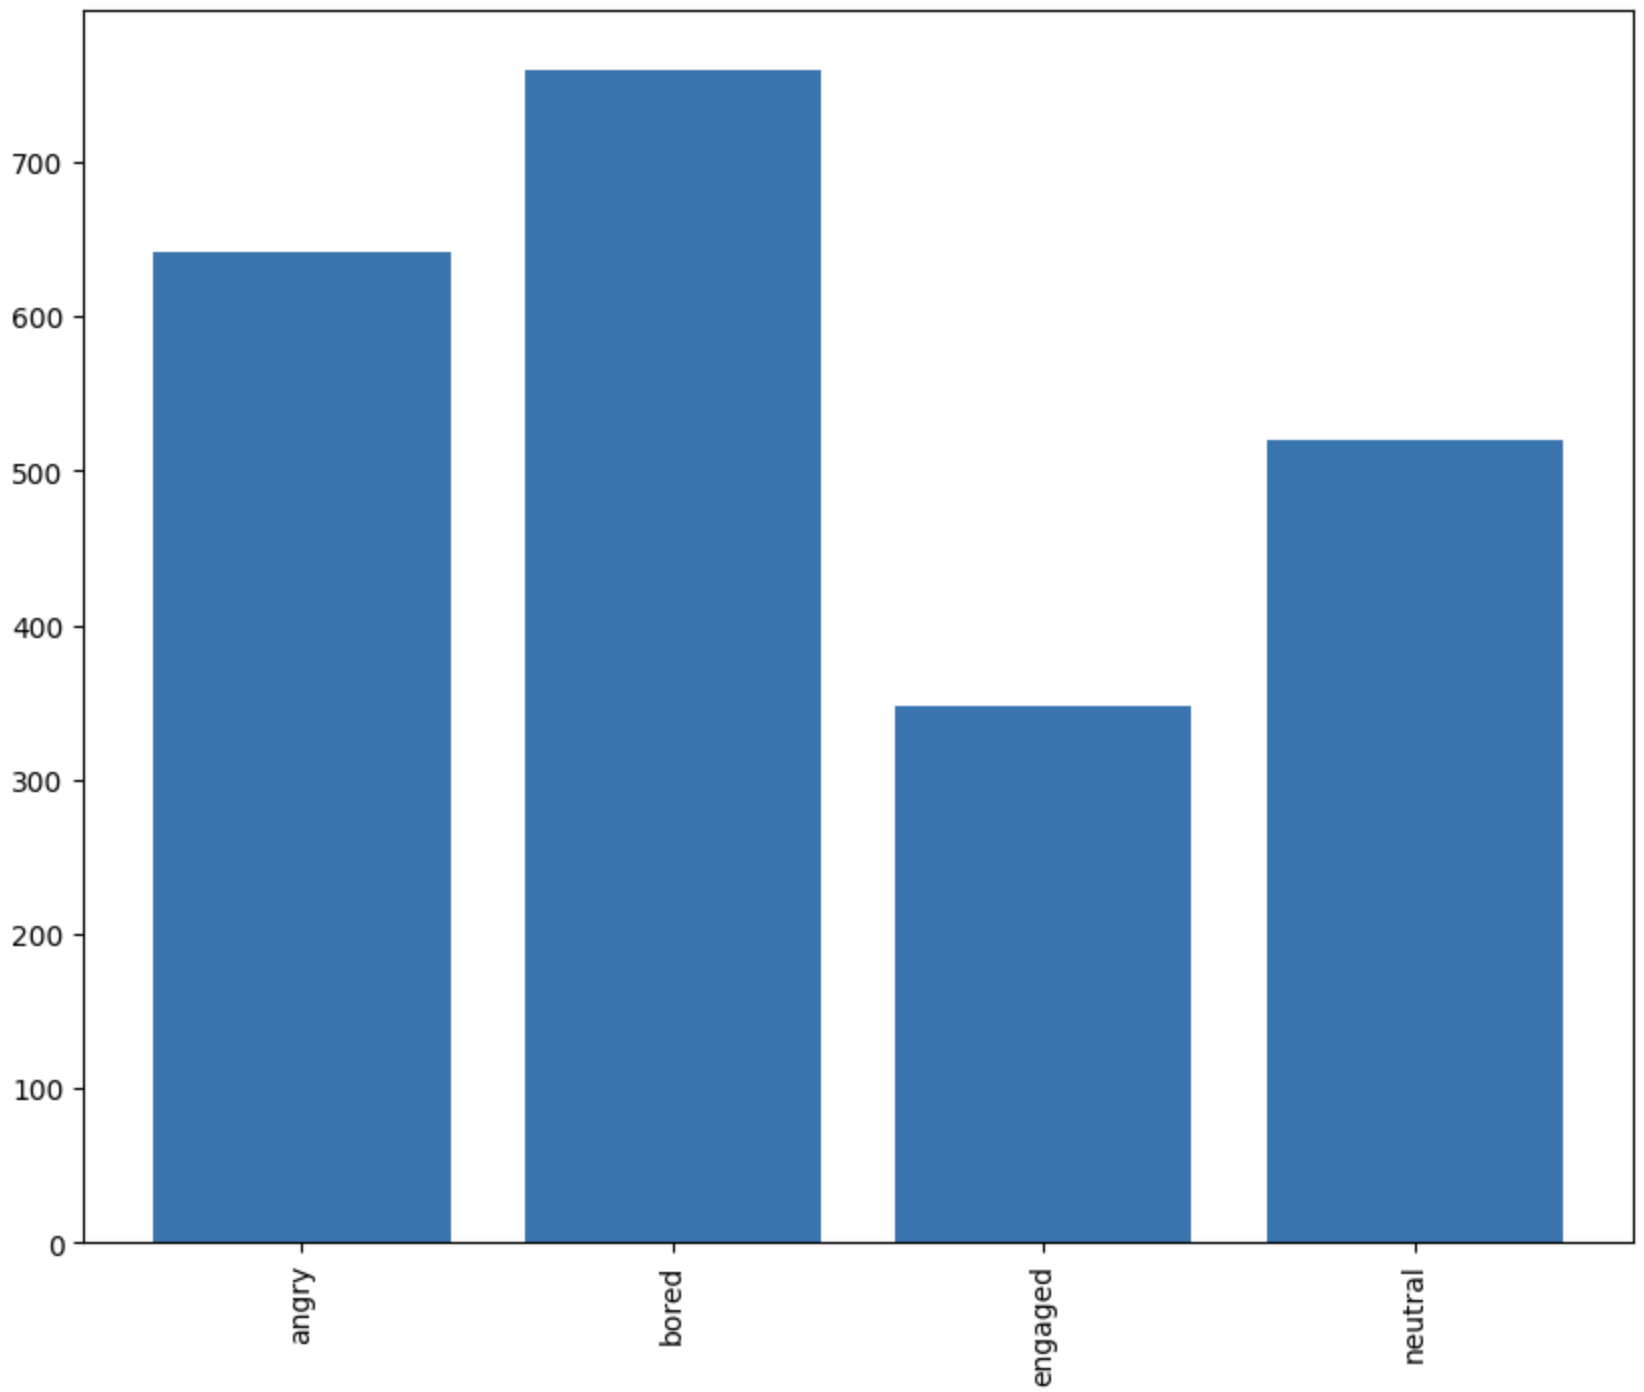
\includegraphics[width=0.7\textwidth, height=6cm]{resources/bg-train.png}
    \caption{Training dataset}
  \end{figure}

  \begin{figure}[h!]
    \centering
    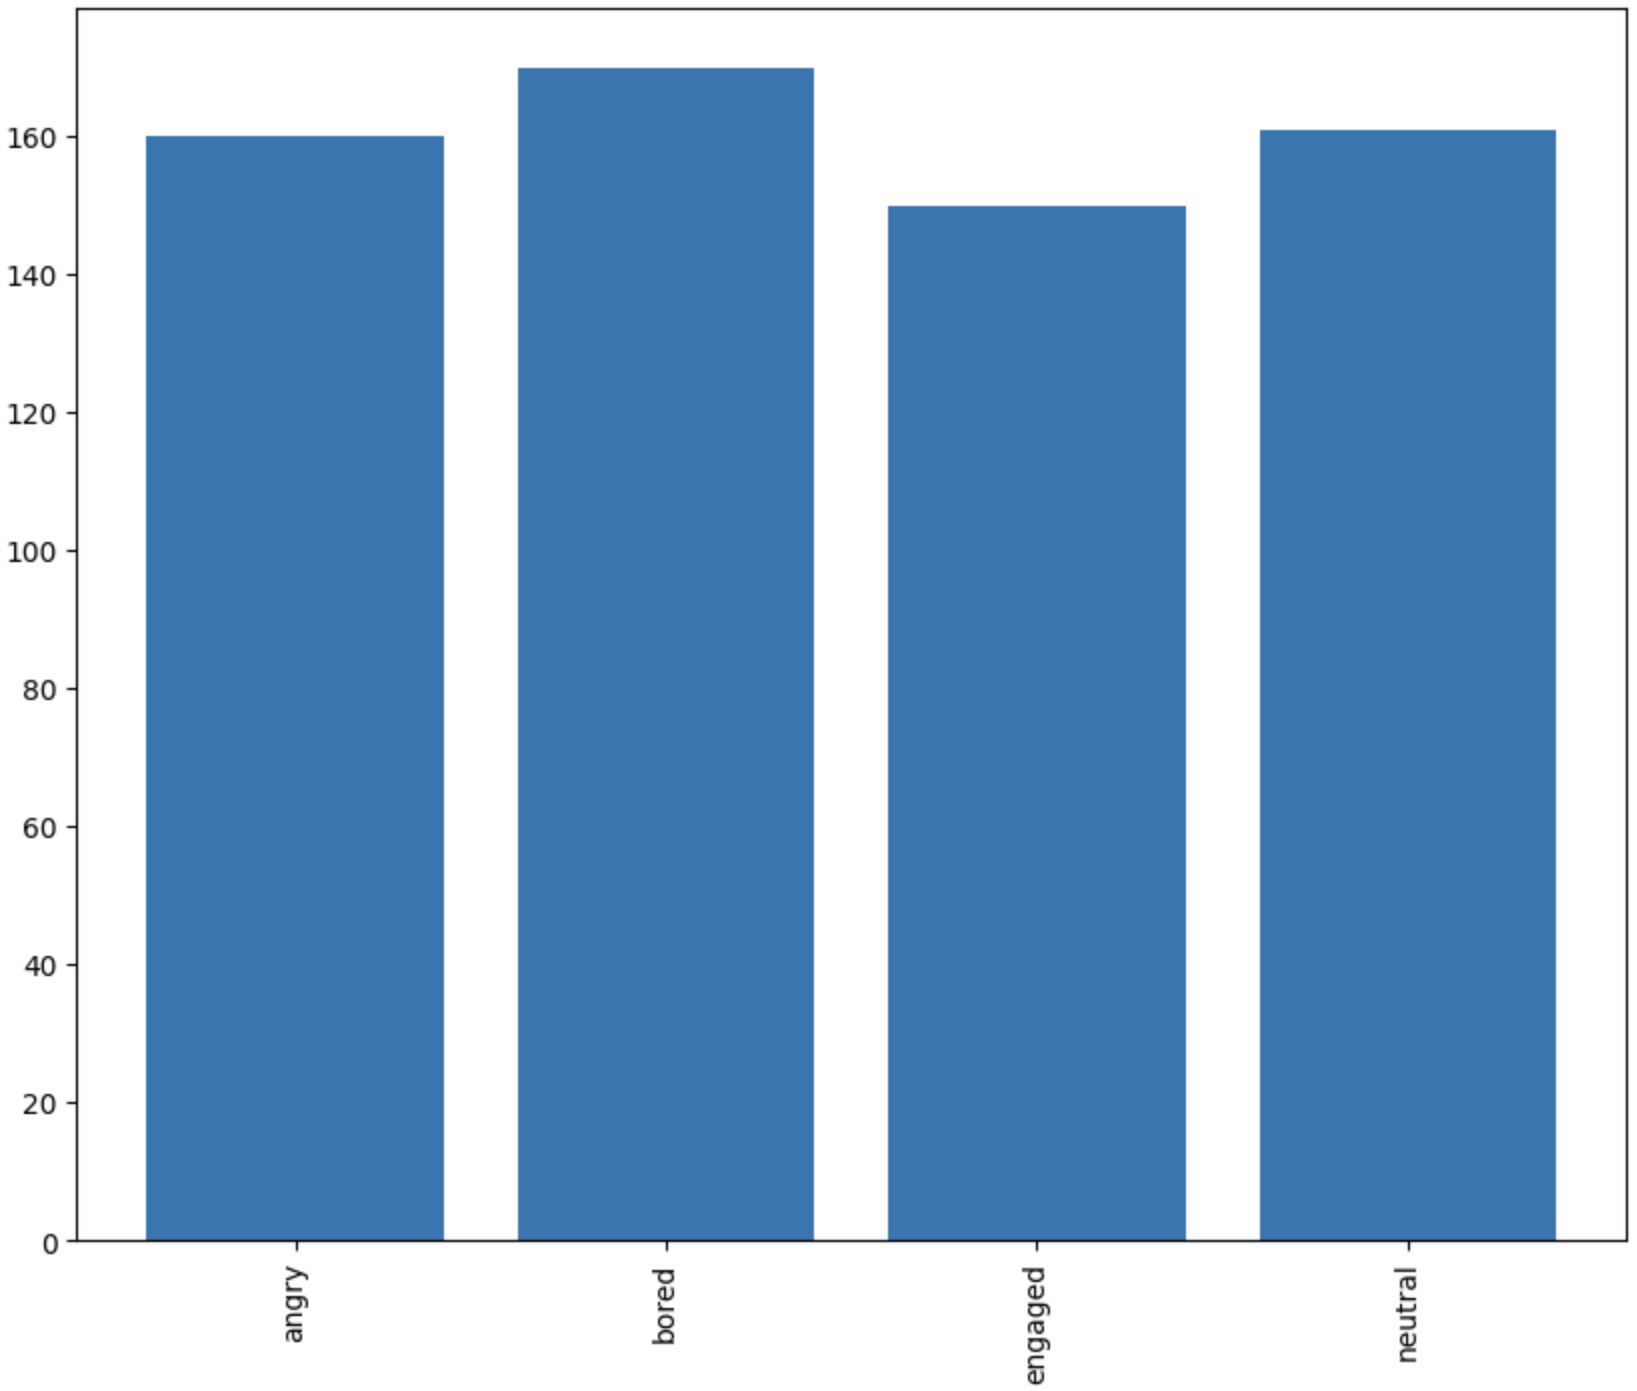
\includegraphics[width=0.7\textwidth, height=6cm]{resources/bg-test.png}
    \caption{Test dataset}
  \end{figure}

\section{Sample Images}

\begin{figure}[h!]
    \centering
    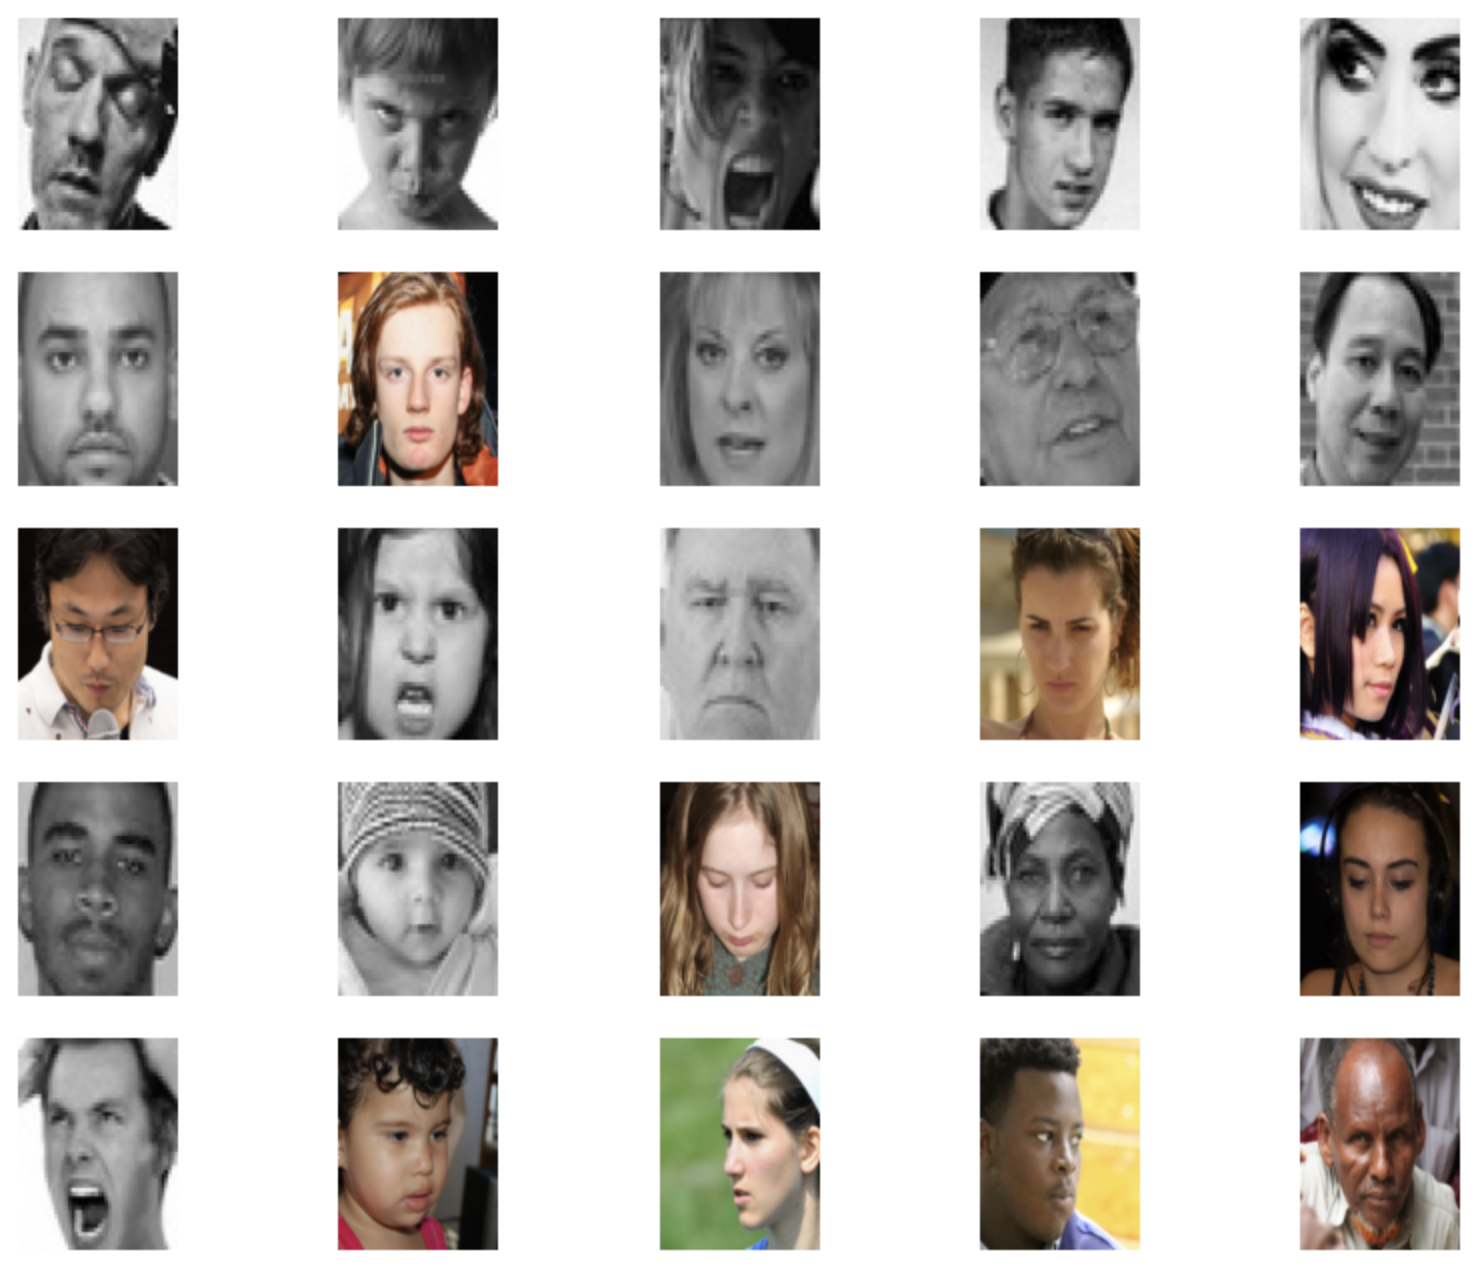
\includegraphics[width=0.9\textwidth, height=8cm]{resources/random25.png}
    \caption{Random set of 25 images from the dataset}
  \end{figure}


\section{Pixel Intensity Distribution}

\begin{figure}[h!]
    \centering
    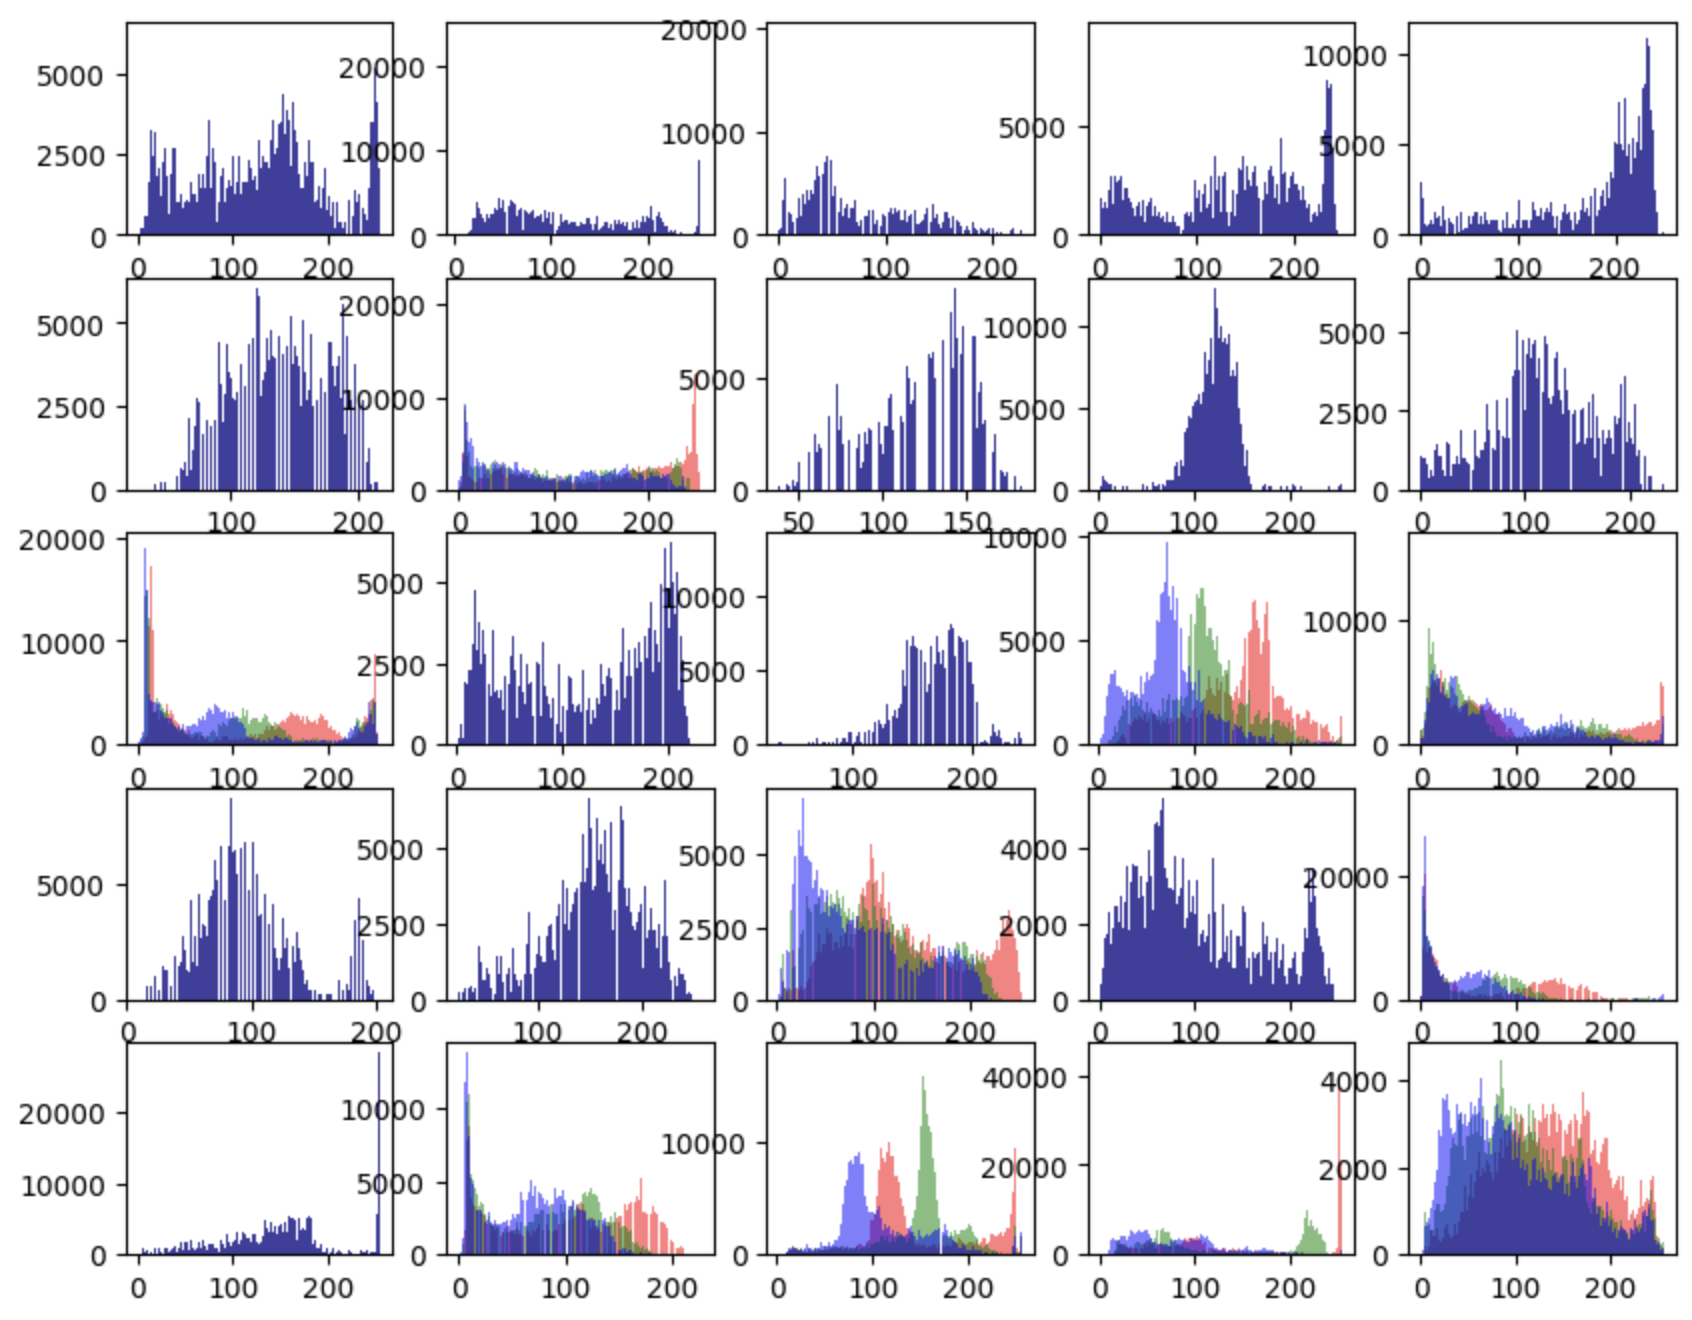
\includegraphics[width=0.9\textwidth, height=8cm]{resources/histo25.png}
    \caption{Distribution of pixel intensities for the images shown above}
  \end{figure}